% This is a template for lecture notes.
\documentclass{article}
\usepackage[UTF8]{ctex}
\usepackage{amssymb}
\usepackage{amsmath}
\usepackage{amsthm}
\usepackage{geometry}
\usepackage{booktabs}
\usepackage{bm}
\usepackage{tcolorbox}
\CTEXoptions[today=old]
%Some commonly used notations
%\geometry{a4paper,bottom = 3cm,left = 3cm, right = 3cm}

%for reference
\usepackage{hyperref}
\usepackage[capitalise]{cleveref}
\crefname{enumi}{}{}

\newtheorem{theorem}{Theorem}
\newtheorem{lemma}[theorem]{Lemma}
\newtheorem{proposition}[theorem]{Proposition}
\newtheorem{corollary}[theorem]{Corollary}
\newtheorem{fact}[theorem]{Fact}
\newtheorem{definition}[theorem]{Definition}
\newtheorem{remark}[theorem]{Remark}
\newtheorem{question}[theorem]{Question}
\newtheorem{answer}[theorem]{Answer}
\newtheorem{exercise}[theorem]{Exercise}
\newtheorem{example}[theorem]{Example}
%\newenvironment{proof}{\noindent \textbf{Proof:}}{$\Box$}
\newtheorem{observation}[theorem]{Observation}

%to use newcommand for convenience
\newcommand\field{\mathbb{F}}
\newcommand\Real{\mathbb{R}}
\newcommand\Q{\mathbb{Q}}
\newcommand\Z{\mathbb{Z}}
\newcommand\complex{\mathbb{C}}

%this is how we define operators.
\DeclareMathOperator{\rank}{rank} % rank

\title{Discussion on Exercise 3}
\author{Ji Jiabao}
\date{\today}

\begin{document}
    \maketitle
    The problem i encountered is that what the image for the endpoint 0,1 should be, 
    since [0,1] is a closed interval while $\mathbb{R}$ is an open interval. 
    But we know there is a simple bijection between (0, 1) and $\mathbb{R}$ with the help of $tan$.
    And from the reading of Was Cantor Surprised, we can take advantage of the injection
    Cantor constructed between [0,1] and [0, 1).\\

    First the simple bijection $f = tan(\frac{\pi}{2} x - \frac{\pi}{2}) (x \in (0, 1))$ between (0, 1) and $\mathbb{R}$.\\
    Next construct the bijection between $(0, 1)$ and [0, 1].

    \begin{figure}[h]
        \centering
        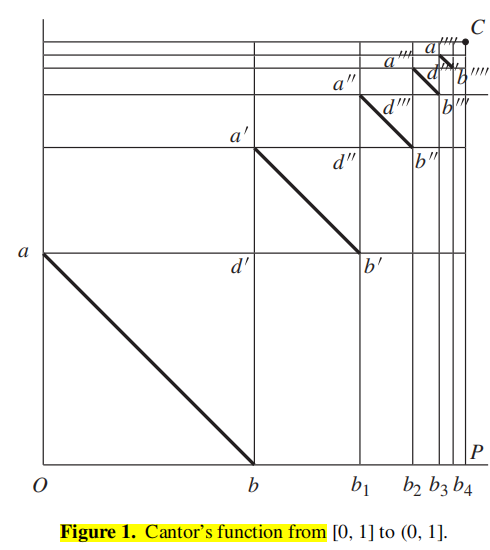
\includegraphics[scale = 0.5]{cantor.png}
        \caption{Cantor's bijection}
    \end{figure}
    "The domain has been divided by a geometric progression, so $b = 1/2$,$ b_1 = 3/4$, and so on;
    $a = (0, 1/2)$, $a' = (1/2, 3/4)$, etc. The point $C$ is (1, 1). The points $d' = (1/2, 1/2)$, $d^{''} = (3/4, 3/4)$, etc. 
    give the corresponding subdivision of the main diagonal." ( I can't explain the curve in english clearly, so i quote the 
    discription in Was Cantor Surprised here). We can slightly change this bijection by ignoring the endpoint C, by doint so, we get 
    the desired bijection $g$.\\
    \hspace*{2em} Also, in a $'modern'$ way(as Cantor would say), we can construct the bijection like this.
    \begin{equation}
        g(x) = \left\{
        \begin{aligned}
            \frac{1}{2} &, & x = 0\\
            \frac{1}{n + 2} &, &(x \in \{\frac{1}{n}, n \in \mathbb{N}\}\\
            x &, &(x \notin \{\frac{1}{n}, n \in \mathbb{N}\})\\
        \end{aligned}
        \right.
    \end{equation}
    By $g$, we map $0, 1, \frac{1}{2}...$ to $\frac{1}{2}, \frac{1}{3}...$, since we have infinite $\frac{1}{n}$ in (0, 1), 
    this can be done.

    To sum up, the bijection between [0, 1] and $\mathbb{R}$ is : $f \circ g$
    





\end{document}